
%% bare_jrnl.tex
%% V1.4b
%% 2015/08/26
%% by Michael Shell
%% see http://www.michaelshell.org/
%% for current contact information.
%%
%% This is a skeleton file demonstrating the use of IEEEtran.cls
%% (requires IEEEtran.cls version 1.8b or later) with an IEEE
%% journal paper.
%%
%% Support sites:
%% http://www.michaelshell.org/tex/ieeetran/
%% http://www.ctan.org/pkg/ieeetran
%% and
%% http://www.ieee.org/

%%*************************************************************************
%% Legal Notice:
%% This code is offered as-is without any warranty either expressed or
%% implied; without even the implied warranty of MERCHANTABILITY or
%% FITNESS FOR A PARTICULAR PURPOSE! 
%% User assumes all risk.
%% In no event shall the IEEE or any contributor to this code be liable for
%% any damages or losses, including, but not limited to, incidental,
%% consequential, or any other damages, resulting from the use or misuse
%% of any information contained here.
%%
%% All comments are the opinions of their respective authors and are not
%% necessarily endorsed by the IEEE.
%%
%% This work is distributed under the LaTeX Project Public License (LPPL)
%% ( http://www.latex-project.org/ ) version 1.3, and may be freely used,
%% distributed and modified. A copy of the LPPL, version 1.3, is included
%% in the base LaTeX documentation of all distributions of LaTeX released
%% 2003/12/01 or later.
%% Retain all contribution notices and credits.
%% ** Modified files should be clearly indicated as such, including  **
%% ** renaming them and changing author support contact information. **
%%*************************************************************************


% *** Authors should verify (and, if needed, correct) their LaTeX system  ***
% *** with the testflow diagnostic prior to trusting their LaTeX platform ***
% *** with production work. The IEEE's font choices and paper sizes can   ***
% *** trigger bugs that do not appear when using other class files.       ***                          ***
% The testflow support page is at:
% http://www.michaelshell.org/tex/testflow/



\documentclass[journal]{IEEEtran}
%
% If IEEEtran.cls has not been installed into the LaTeX system files,
% manually specify the path to it like:
% \documentclass[journal]{../sty/IEEEtran}
\usepackage[dvipdfmx]{graphicx}
\usepackage{mathrsfs}
\usepackage{mathtools}
\usepackage{comment}
\usepackage{amsmath,amssymb}
\usepackage{ascmac}
\usepackage{bm}
\usepackage{cite}
\usepackage{nidanfloat}
\usepackage{url}
\usepackage{color}

\def\rnum#1{\expandafter{\romannumeral #1}}

\newcommand{\argmin}{\mathop{\rm arg~min}\limits}
\newcommand{\argmax}{\mathop{\rm arg~max}\limits}
  \newcommand{\Tabref}[1]{表~\ref{#1}}
  \newcommand{\Equref}[1]{式~(\ref{#1})}
  \newcommand{\Figref}[1]{図~\ref{#1}}





% Some very useful LaTeX packages include:
% (uncomment the ones you want to load)


% *** MISC UTILITY PACKAGES ***
%
%\usepackage{ifpdf}
% Heiko Oberdiek's ifpdf.sty is very useful if you need conditional
% compilation based on whether the output is pdf or dvi.
% usage:
% \ifpdf
%   % pdf code
% \else
%   % dvi code
% \fi
% The latest version of ifpdf.sty can be obtained from:
% http://www.ctan.org/pkg/ifpdf
% Also, note that IEEEtran.cls V1.7 and later provides a builtin
% \ifCLASSINFOpdf conditional that works the same way.
% When switching from latex to pdflatex and vice-versa, the compiler may
% have to be run twice to clear warning/error messages.






% *** CITATION PACKAGES ***
%
%\usepackage{cite}
% cite.sty was written by Donald Arseneau
% V1.6 and later of IEEEtran pre-defines the format of the cite.sty package
% \cite{} output to follow that of the IEEE. Loading the cite package will
% result in citation numbers being automatically sorted and properly
% "compressed/ranged". e.g., [1], [9], [2], [7], [5], [6] without using
% cite.sty will become [1], [2], [5]--[7], [9] using cite.sty. cite.sty's
% \cite will automatically add leading space, if needed. Use cite.sty's
% noadjust option (cite.sty V3.8 and later) if you want to turn this off
% such as if a citation ever needs to be enclosed in parenthesis.
% cite.sty is already installed on most LaTeX systems. Be sure and use
% version 5.0 (2009-03-20) and later if using hyperref.sty.
% The latest version can be obtained at:
% http://www.ctan.org/pkg/cite
% The documentation is contained in the cite.sty file itself.






% *** GRAPHICS RELATED PACKAGES ***
%
\ifCLASSINFOpdf
  % \usepackage[pdftex]{graphicx}
  % declare the path(s) where your graphic files are
  % \graphicspath{{../pdf/}{../jpeg/}}
  % and their extensions so you won't have to specify these with
  % every instance of \includegraphics
  % \DeclareGraphicsExtensions{.pdf,.jpeg,.png}
\else
  % or other class option (dvipsone, dvipdf, if not using dvips). graphicx
  % will default to the driver specified in the system graphics.cfg if no
  % driver is specified.
  % \usepackage[dvips]{graphicx}
  % declare the path(s) where your graphic files are
  % \graphicspath{{../eps/}}
  % and their extensions so you won't have to specify these with
  % every instance of \includegraphics
  % \DeclareGraphicsExtensions{.eps}
\fi
% graphicx was written by David Carlisle and Sebastian Rahtz. It is
% required if you want graphics, photos, etc. graphicx.sty is already
% installed on most LaTeX systems. The latest version and documentation
% can be obtained at: 
% http://www.ctan.org/pkg/graphicx
% Another good source of documentation is "Using Imported Graphics in
% LaTeX2e" by Keith Reckdahl which can be found at:
% http://www.ctan.org/pkg/epslatex
%
% latex, and pdflatex in dvi mode, support graphics in encapsulated
% postscript (.eps) format. pdflatex in pdf mode supports graphics
% in .pdf, .jpeg, .png and .mps (metapost) formats. Users should ensure
% that all non-photo figures use a vector format (.eps, .pdf, .mps) and
% not a bitmapped formats (.jpeg, .png). The IEEE frowns on bitmapped formats
% which can result in "jaggedy"/blurry rendering of lines and letters as
% well as large increases in file sizes.
%
% You can find documentation about the pdfTeX application at:
% http://www.tug.org/applications/pdftex





% *** MATH PACKAGES ***
%
%\usepackage{amsmath}
% A popular package from the American Mathematical Society that provides
% many useful and powerful commands for dealing with mathematics.
%
% Note that the amsmath package sets \interdisplaylinepenalty to 10000
% thus preventing page breaks from occurring within multiline equations. Use:
%\interdisplaylinepenalty=2500
% after loading amsmath to restore such page breaks as IEEEtran.cls normally
% does. amsmath.sty is already installed on most LaTeX systems. The latest
% version and documentation can be obtained at:
% http://www.ctan.org/pkg/amsmath





% *** SPECIALIZED LIST PACKAGES ***
%
%\usepackage{algorithmic}
% algorithmic.sty was written by Peter Williams and Rogerio Brito.
% This package provides an algorithmic environment fo describing algorithms.
% You can use the algorithmic environment in-text or within a figure
% environment to provide for a floating algorithm. Do NOT use the algorithm
% floating environment provided by algorithm.sty (by the same authors) or
% algorithm2e.sty (by Christophe Fiorio) as the IEEE does not use dedicated
% algorithm float types and packages that provide these will not provide
% correct IEEE style captions. The latest version and documentation of
% algorithmic.sty can be obtained at:
% http://www.ctan.org/pkg/algorithms
% Also of interest may be the (relatively newer and more customizable)
% algorithmicx.sty package by Szasz Janos:
% http://www.ctan.org/pkg/algorithmicx




% *** ALIGNMENT PACKAGES ***
%
%\usepackage{array}
% Frank Mittelbach's and David Carlisle's array.sty patches and improves
% the standard LaTeX2e array and tabular environments to provide better
% appearance and additional user controls. As the default LaTeX2e table
% generation code is lacking to the point of almost being broken with
% respect to the quality of the end results, all users are strongly
% advised to use an enhanced (at the very least that provided by array.sty)
% set of table tools. array.sty is already installed on most systems. The
% latest version and documentation can be obtained at:
% http://www.ctan.org/pkg/array


% IEEEtran contains the IEEEeqnarray family of commands that can be used to
% generate multiline equations as well as matrices, tables, etc., of high
% quality.




% *** SUBFIGURE PACKAGES ***
%\ifCLASSOPTIONcompsoc
%  \usepackage[caption=false,font=normalsize,labelfont=sf,textfont=sf]{subfig}
%\else
%  \usepackage[caption=false,font=footnotesize]{subfig}
%\fi
% subfig.sty, written by Steven Douglas Cochran, is the modern replacement
% for subfigure.sty, the latter of which is no longer maintained and is
% incompatible with some LaTeX packages including fixltx2e. However,
% subfig.sty requires and automatically loads Axel Sommerfeldt's caption.sty
% which will override IEEEtran.cls' handling of captions and this will result
% in non-IEEE style figure/table captions. To prevent this problem, be sure
% and invoke subfig.sty's "caption=false" package option (available since
% subfig.sty version 1.3, 2005/06/28) as this is will preserve IEEEtran.cls
% handling of captions.
% Note that the Computer Society format requires a larger sans serif font
% than the serif footnote size font used in traditional IEEE formatting
% and thus the need to invoke different subfig.sty package options depending
% on whether compsoc mode has been enabled.
%
% The latest version and documentation of subfig.sty can be obtained at:
% http://www.ctan.org/pkg/subfig




% *** FLOAT PACKAGES ***
%
%\usepackage{fixltx2e}
% fixltx2e, the successor to the earlier fix2col.sty, was written by
% Frank Mittelbach and David Carlisle. This package corrects a few problems
% in the LaTeX2e kernel, the most notable of which is that in current
% LaTeX2e releases, the ordering of single and double column floats is not
% guaranteed to be preserved. Thus, an unpatched LaTeX2e can allow a
% single column figure to be placed prior to an earlier double column
% figure.
% Be aware that LaTeX2e kernels dated 2015 and later have fixltx2e.sty's
% corrections already built into the system in which case a warning will
% be issued if an attempt is made to load fixltx2e.sty as it is no longer
% needed.
% The latest version and documentation can be found at:
% http://www.ctan.org/pkg/fixltx2e


%\usepackage{stfloats}
% stfloats.sty was written by Sigitas Tolusis. This package gives LaTeX2e
% the ability to do double column floats at the bottom of the page as well
% as the top. (e.g., "\begin{figure*}[!b]" is not normally possible in
% LaTeX2e). It also provides a command:
%\fnbelowfloat
% to enable the placement of footnotes below bottom floats (the standard
% LaTeX2e kernel puts them above bottom floats). This is an invasive package
% which rewrites many portions of the LaTeX2e float routines. It may not work
% with other packages that modify the LaTeX2e float routines. The latest
% version and documentation can be obtained at:
% http://www.ctan.org/pkg/stfloats
% Do not use the stfloats baselinefloat ability as the IEEE does not allow
% \baselineskip to stretch. Authors submitting work to the IEEE should note
% that the IEEE rarely uses double column equations and that authors should try
% to avoid such use. Do not be tempted to use the cuted.sty or midfloat.sty
% packages (also by Sigitas Tolusis) as the IEEE does not format its papers in
% such ways.
% Do not attempt to use stfloats with fixltx2e as they are incompatible.
% Instead, use Morten Hogholm'a dblfloatfix which combines the features
% of both fixltx2e and stfloats:
%
% \usepackage{dblfloatfix}
% The latest version can be found at:
% http://www.ctan.org/pkg/dblfloatfix




%\ifCLASSOPTIONcaptionsoff
%  \usepackage[nomarkers]{endfloat}
% \let\MYoriglatexcaption\caption
% \renewcommand{\caption}[2][\relax]{\MYoriglatexcaption[#2]{#2}}
%\fi
% endfloat.sty was written by James Darrell McCauley, Jeff Goldberg and 
% Axel Sommerfeldt. This package may be useful when used in conjunction with 
% IEEEtran.cls'  captionsoff option. Some IEEE journals/societies require that
% submissions have lists of figures/tables at the end of the paper and that
% figures/tables without any captions are placed on a page by themselves at
% the end of the document. If needed, the draftcls IEEEtran class option or
% \CLASSINPUTbaselinestretch interface can be used to increase the line
% spacing as well. Be sure and use the nomarkers option of endfloat to
% prevent endfloat from "marking" where the figures would have been placed
% in the text. The two hack lines of code above are a slight modification of
% that suggested by in the endfloat docs (section 8.4.1) to ensure that
% the full captions always appear in the list of figures/tables - even if
% the user used the short optional argument of \caption[]{}.
% IEEE papers do not typically make use of \caption[]'s optional argument,
% so this should not be an issue. A similar trick can be used to disable
% captions of packages such as subfig.sty that lack options to turn off
% the subcaptions:
% For subfig.sty:
% \let\MYorigsubfloat\subfloat
% \renewcommand{\subfloat}[2][\relax]{\MYorigsubfloat[]{#2}}
% However, the above trick will not work if both optional arguments of
% the \subfloat command are used. Furthermore, there needs to be a
% description of each subfigure *somewhere* and endfloat does not add
% subfigure captions to its list of figures. Thus, the best approach is to
% avoid the use of subfigure captions (many IEEE journals avoid them anyway)
% and instead reference/explain all the subfigures within the main caption.
% The latest version of endfloat.sty and its documentation can obtained at:
% http://www.ctan.org/pkg/endfloat
%
% The IEEEtran \ifCLASSOPTIONcaptionsoff conditional can also be used
% later in the document, say, to conditionally put the References on a 
% page by themselves.




% *** PDF, URL AND HYPERLINK PACKAGES ***
%
%\usepackage{url}
% url.sty was written by Donald Arseneau. It provides better support for
% handling and breaking URLs. url.sty is already installed on most LaTeX
% systems. The latest version and documentation can be obtained at:
% http://www.ctan.org/pkg/url
% Basically, \url{my_url_here}.




% *** Do not adjust lengths that control margins, column widths, etc. ***
% *** Do not use packages that alter fonts (such as pslatex).         ***
% There should be no need to do such things with IEEEtran.cls V1.6 and later.
% (Unless specifically asked to do so by the journal or conference you plan
% to submit to, of course. )


% correct bad hyphenation here
\hyphenation{op-tical net-works semi-conduc-tor}


\begin{document}
%
% paper title
% Titles are generally capitalized except for words such as a, an, and, as,
% at, but, by, for, in, nor, of, on, or, the, to and up, which are usually
% not capitalized unless they are the first or last word of the title.
% Linebreaks \\ can be used within to get better formatting as desired.
% Do not put math or special symbols in the title.
\title{Utility Based Scheduling for Multi-UAV Search System in Disaster Scenarios}
%
%
% author names and IEEE memberships
% note positions of commas and nonbreaking spaces ( ~ ) LaTeX will not break
% a structure at a ~ so this keeps an author's name from being broken across
% two lines.
% use \thanks{} to gain access to the first footnote area
% a separate \thanks must be used for each paragraph as LaTeX2e's \thanks
% was not built to handle multiple paragraphs
%

%\author{Michael~Shell,~\IEEEmembership{Member,~IEEE,}
%        John~Doe,~\IEEEmembership{Fellow,~OSA,}
%        and~Jane~Doe,~\IEEEmembership{Life~Fellow,~IEEE}% <-this % stops a space
\author{Kosei MIYANO,Ryoichi SHINKUMA,Eiji OKI, and Takehiro SATO
\thanks{K. Miyano, R. Shinkuma, E. OKI, and T. SATO are with Graduate School of
Informatics,Kyoto University,Yoshidahon-machi, Sakyo-ku, Kyoto-shi,
Kyoto, Japan, 606-8501.
e-mail: (kmiyano@icn.cce.i.kyoto-u.ac.jp, \{shinkuma, oki, takehiro.sato\}@i.kyoto-u.ac.jp)}}
%\thanks{M. Shell was with the Departmentof Electrical and Computer Engineering, Georgia Institute of Technology, Atlanta,GA, 30332 USA e-mail: (see http://www.michaelshell.org/contact.html).}% <-this % stops a space
%thanks{J. Doe and J. Doe are with Anonymous University.}% <-this % stops a space
%\thanks{Manuscript received April 19, 2005; revised August 26, 2015.}}

% note the % following the last \IEEEmembership and also \thanks - 
% these prevent an unwanted space from occurring between the last author name
% and the end of the author line. i.e., if you had this:
% 
% \author{....lastname \thanks{...} \thanks{...} }
%                     ^------------^------------^----Do not want these spaces!
%
% a space would be appended to the last name and could cause every name on that
% line to be shifted left slightly. This is one of those "LaTeX things". For
% instance, "\textbf{A} \textbf{B}" will typeset as "A B" not "AB". To get
% "AB" then you have to do: "\textbf{A}\textbf{B}"
% \thanks is no different in this regard, so shield the last } of each \thanks
% that ends a line with a % and do not let a space in before the next \thanks.
% Spaces after \IEEEmembership other than the last one are OK (and needed) as
% you are supposed to have spaces between the names. For what it is worth,
% this is a minor point as most people would not even notice if the said evil
% space somehow managed to creep in.



% The paper headers
\markboth{IEEE sensors Journal,~Vol.~14, No.~8, August~2018}%
{Shell \MakeLowercase{\textit{et al.}}: Bare Demo of IEEEtran.cls for IEEE Journals}
% The only time the second header will appear is for the odd numbered pages
% after the title page when using the twoside option.
% 
% *** Note that you probably will NOT want to include the author's ***
% *** name in the headers of peer review papers.                   ***
% You can use \ifCLASSOPTIONpeerreview for conditional compilation here if
% you desire.




% If you want to put a publisher's ID mark on the page you can do it like
% this:
%\IEEEpubid{0000--0000/00\$00.00~\copyright~2015 IEEE}
% Remember, if you use this you must call \IEEEpubidadjcol in the second
% column for its text to clear the IEEEpubid mark.



% use for special paper notices
%\IEEEspecialpapernotice{(Invited Paper)}


% make the title area
\maketitle

% As a general rule, do not put math, special symbols or citations
% in the abstract or keywords.

% For peer review papers, you can put extra information on the cover
% page as needed:
% \ifCLASSOPTIONpeerreview
% \begin{center} \bfseries EDICS Category: 3-BBND \end{center}
% \fi
%
% For peerreview papers, this IEEEtran command inserts a page break and
% creates the second title. It will be ignored for other modes.
\IEEEpeerreviewmaketitle

\begin{abstract}
%The number of deaths and missing people due to natural disasters is still a big social issue these days in many countries.
%It is a still big social issue these days to find people who have disappeared because of getting lost in unexpected situation like disaster.
%To search such lost people in disaster-damaged areas, the integrated system of the mobility of multiple unmanned aerial vehicles (UAVs) has been studied as a promising solution for that.
Micro or small unmanned aerial vehicles (UAVs) is a promising solution for finding people who have disappeared because of getting lost in unexpected situation like disaster.
It takes long time to analyze the acquired image data for the target recognition due to the limited computational resource of small UAVs.
In addition, the data transfer time can increase in the disaster-hit areas due to the  damage of communication infrastructures.
However, the prior researches did not consider both processing time of the acquired data and data transfer time, despite the temporal requirement in the surveillance scenarios.
Therefore, this paper proposes a scheduling method of multi-UAV search system that considers processing time of image data and data transfer time.
We present the utility-based problem formulation that ensures the freshness of individual obtained piece of information while obtaining as many pieces of information as possible for a certain period.
Simulation results verify that the proposed scheduling method ensures the freshness of individual obtained piece of information while delivering as many pieces of information as possible for a certain period by evaluating each information in terms of two metrics: i) elapsed time from start time and ii) elapsed time after acquired.
\end{abstract}
\begin{IEEEkeywords}
uav (unmanned aerial vehicle), target search, scheduling, edge computing
\end{IEEEkeywords}

%\vspace*{-3mm}

\section{introduction}\label{intro}
The number of deaths and missing people due to natural disasters is still a serious problem in many countries.
According to a report by Centre for Research on the Epidemiology of Disasters\cite{CRED2016}, the average number of deaths and missing people due to natural disasters occurred all over the world, such as earthquakes, hurricanes, forest fires, and floods, from 2006 to 2015 was approximately 70,000.
In order to reduce the number, one of the solutions to reduce the number is to increase the number of rescue teams.
The report by Japan Ministry of Defense after the great east Japan earthquake suggests that  it is necessary to secure manpower through guidelines for the concentration of units in the immediate aftermath of a disaster.
%and by improving the vacancy fillrate for frontline units.
%そういった人員の確保においては,莫大な予算及び二次遭難のリスク課題となる.
However, a huge budget is required to secure manpower and the risk of secondary damages in disaster occurrence areas is serious remaining issues to be solved\cite{disaster2011}.

Micro or small unmanned aerial vehicles (UAVs), also known as
drones, are expected to be emerging solutions to solve the above problem in areas where humans and ground vehicles cannot easily step into like disaster-damaged areas.
Technological advances in the recent years have led to the emergence of smaller and cheaper UAVs, which have some functions such as transporting relief supplies, collecting data by using equipped sensors and operating as adhoc wireless mesh network infrastructure in such isolated areas \cite{Andre2014,Erdelj2016,Felice2014}.
Collecting image data is especially important because it is applicable to many use cases such as search and rescue mission, fire detection and surveilance.
%いずれも時間的制約があるシチュエーションなので,できる限り早くsensor dataを集める必要がある.
Since  there are time constraints in such situations, UAVs need to collect sensor data as soon as possible.
%東日本大震災においても,時間が経つにつれて,The number of deaths and missing peopleは急激に増大した.
In the great east Japan earthquake, as time passed, the number of deaths and missing people  dramatically increased\cite{japan2011}.

%従来研究では信頼性, ロバスト性, 効率性などをより一層向上させるため, UAVを複数用いたsurveilanceの研究が盛んに行われて来たIn the previous works, 
Surveillance using multiple UAVs has been receiving increasing attention for reasons such as increase in system reliability, robustness, and efficiency\cite{Lanillos2014,Maza2007,Meng2014,chang2016,Mirzaei2011}.
%しかし,いずれにおいてもUAVがimage dataを取得したら即座にユーザも必要な情報が得られるとしており,時間的な要求条件があるにも関わらず,image dataの処理時間とデータ転送時間の二点が考慮されていない.
However, despite the temporal requirement in these surveillance systems, it is assumed that the user can obtain necessary information as soon as UAV acquires image data: both processing time of image data and data transfer time are not taken into consideration. In the practical situation, it takes long time to analyze images for target recognition due to the limited computational resource of small UAVs. In addition, the data transfer time can increase in the disaster-hit areas due to the damage of communication infrastructures.
%以上を踏まえ本稿では, センシング後のUAVとエッジによる計算時間を考慮し人命救助を行うユーザのutilityを最大化するUAVのスケジューリング方式を提案する.本提案方式ではutilityの指標として, 捜索結果を実際にユーザが取得する効率(以下, 取得効率)とユーザが取得する間隔(以下, 取得間隔)の二点を統合した指標を用いる.

Therefore, this paper proposes a scheduling method of multi-UAV search system that considers processing time of image data and data transfer time.
We present the problem formulation of the proposed scheduling method that maximizes the user’s utility, which is calculated from the efficiency of obtaining results from analyzed data and the interval of obtaining the results.
We show the results of performance evaluation to verify that the proposed method ensures the freshness of individual obtained piece of information while delivering as many pieces of information as possible for a certain period.

The remainder of this paper is organized as follows. Section II discusses the related work. Section III presents the system overview and proposed scheduling method. Section IV then provides the performance evaluation of the proposed method through a simulation, followed by the extension to two-dimensional model in Section V. Finally, Section VI concludes this paper.
%
%
%
%
%
%
%
%
%
%
%
%
\section{Related work}
This section discusses the prior works related to this paper.
First we will discuss UAV Applications in disaster areas. 
Among the application scenarios that will be introduced in Section \ref{app}, data collection using equipped sensors is carried out in our system.
Next the prior researches on Multi-UAV cooperation for area coverage is discussed since it is also assumed in our search system as mentioned in Section \ref{intro}.
Finally, we also discuss prior works on inter UAV cooperation for computing and  computing on UAVs with edge computing.
In our system, it is assumed that the collected data is processed locally onboard UAVs with edge computing but inter UAV cooperation for computing is not considered since the overhead of transmission between UAVs is large and is out of the scope of this paper.

\subsection{UAV Applications in disaster areas}\label{app}
Transporting relief supplies by UAVs is very important since there is a possibility that humans and ground vehicles cannot easily step into the disaster areas.
Bamburry mentioned the ability of a UAV to deliver medical products to remote and hard-to-reach areas\cite{Bamburry2015}.
For example, in the devastating 2010 earthquake in Haiti, a UAV delivery system was used to deliver medicine to camps set up after the disaster\cite{May2015}.

UAVs can also collect data by using equipped sensors. In \cite{Wada2015}, Each UAV is provided with a mobile optical sensors and image transmission modules developed by the Wada et al. The optical sensor which is a combination of a IR sensor and a visible-light sensor enables data collection even at night or against smoke in the disaster areas.
After the launch, a UAV executes auto flight along the way points by recognizing its positions and  obtains the necessary video/image information. The UAV transmits it to the server and shares it with users via the Internet.

UAVs also often operate as adhoc wireless mesh network infrastructure, which is called Flying Ad Hoc Networks (FANET)\cite{Bekmezci2013}.
In 2016, S\'anchez et al. aim to provide connectivity for rescuers and disaster victims using UAVs\cite{Garcia2016}.
They propose a Jaccard-based movement rules to define the UAVs best positions for providing the best communication service to the victims in a urban disaster scenario.
Finally they compare among several local search computational intelligence algorithms implemented such as simulated annealing, hill climbing, and random walk for deciding the best tactical UAV movements.

\subsection{Multi-UAV cooperation for area coverage}\label{cover}
Maza et al. provided a pioneer work in cooperatively searching a given area to detect objects of interest by UAVs\cite{Maza2007}.
First they determine relative capabilities of each UAV, based on factors like flight speed, altitude required for the mission, sensitivity to wind conditions and sensing width.
Then, they divide the whole area by divide-and-conquer, taking into account the UAV’s relative capabilities and initial locations.
Finally, they set the waypoints of each UAV so that the number of turns needed along a zigzag pattern is minimized.

Zhao et al. in 2016 tackled the challenging problem of not only searching the target area for a lost target but also tracking the target\cite{chang2016}.
In the tracking stage, each UAV keeps desired distance with the target, coordinating the angular separation between neighboring UAVs to the same angle.
if there is a shelter between UAV and target, the target state is predicted by the target model with the former target information.  
In the searching stage, multi-UAVs divide the search region equally which is determined by the target lost duration time and speed and then search for the target by the method of shrinking annulus.
The switch tactics between the tracking stage and the searching stage was also proposed. 

In 2017, Hayat et al. proposed a multi-objective optimization algorithm to search and plan paths for UAVs\cite{Hayat 2017}.
UAVs search for the target cooperatively and soon after some UAV detects the target, the other UAVs takes positions for relay chain formation between the UAV and a base station.
The algorithm aims to minimize the mission completion time, which includes the time to find the target and the time to setup a communication path.
Finally they compare among three strategies that perform search by UAVs in a similar manner but have a different path planning in terms of the mission completion time.

\subsection{Multi-UAV cooperation for computing}\label{compute}
UAV Applications in disaster areas require UAVs to deal with intensive computation tasks such as image/video processing, pattern recognition and feature extraction. 
Computation offloading is very important since computational power of a single UAV is limited.
\subsubsection{inter UAV cooperation}
Ouahouah et al. in 2017 proposed the use of offloading mechanism among UAVs equipped with IoT devices\cite{Ouahouah2017}.
Each IoT task is partitioned into a set of sub-tasks that can be executed simultaneously among a cluster of UAVs.
The sub-tasks is assigned to UAVs based on their power supply, resources in terms of memory and CPU computation, and their on-board IoT devices.
Two solutions were proposed for  computation offloading:Energy aware optimal task offloading and Delay aware optimal task offloading.
The former maximizes the UAVs lifetime by electing the UAVs with higher power supply.
The latter reduces the response time by favoring the selection of UAVs with more resource capacities.

In 2018, Valentino et al. proposed an opportunistic and adaptive computational offloading scheme between UAV clusters\cite{Valentino2018}.
A cluster head will broadcast a ‘hello’ message indicating their presence and available resources and then a local cluster send an offloading request to a desired cluster head.
a local cluster decides if it is better to do the task alone or to offload, estimating response time for doing the computational offloading and processing the given task through computing power, size of task, bandwidth, and data rate of wireless network.

\subsubsection{Edge computing}
Edge computing has been proposed as an effective mean of supplementing computational resources for UAVs\cite{Motlagh2017,Messous2017}.

Motlagh et al. in 2017 demonstrated how UAVs can be used for crowd surveillance based on face recognition. 
Due to the computational overhead required by such a use case and given the limited power supply of UAVs, they performed the offloading of video data processing to a mobile edge computing node.
The obtained results showed clearly the benefits of computation offloading compared to the local processing of video data onboard UAVs in saving energy and quickly detecting and recognizing suspicious persons in a crowd.

Messous et al. in 2017 tackled a computation offloading problem with three different devices:UAV, base station and edge server, which carry out the heavy computation tasks.
They prove the existence of a Nash Equilibrium and design an offloading algorithm that converges to the optimal point.
Their cost function was defined as a combination of two performance metrics: energy and delay.
They finally achieved better value of the utility using the the offloading algorithm, compared to computing on: edge server, base station and drone respectively.
%
%
%
%
%
%
%
%
%
%
%
%
%

\section{Proposed method}\label{method}

\subsection{System overview}\label{sys}
\subsubsection{System model}\label{sysmo}

\begin{figure}[t]
\begin{center}
\includegraphics[width=8.0cm]{fig/newmodel.eps}
%\vspace{-2.5mm}
\caption{System illustration}
%\vspace{-2.5mm}
\label{model}
\end{center}
\end{figure}

Figure \ref{model} depicts the system model we assume in this paper. 
The system consists of a user device (UD), multiple UAVs, and an edge server (ES), the roles of which are described as below.
%
The UD is the central operating entity in the system and operates all the UAVs and the ES; the UD determines flying routes and timings of UAVs and assigns workloads of computing sensor data to UAVs and the ES.
%
The UD also works to forward sensor data received from UAVs to the ES and to obtain computational results from both UAVs and the ES.

Each UAV is operated by the UD and performs the following actions autonomously in the distributed manner.
%
(I) Flying between the initial position, at which the UAV can communicate directly with the UD, and the sensing region assigned to the UAV 
(I\hspace{-.1em}I) Acquiring image data (still or moving images) of the sensing region assigned to the UAV.
(I\hspace{-.1em}I\hspace{-.1em}I) Staying at the initial position and performing the following actions in parallel: (a) analyzing a part of collected image data with the computational power of the UAV and (b) delegating the analysis of the rest of the data to the ES.
(I\hspace{-.1em}V) Reporting results obtained from the analysis of image data to the UD soon after it has been completed.
%
Note that we assume that UAVs cannot perform any analysis while flying; computational resources of UAVs are fully used for flight control and image acquiring during the flight.Each UAV repeats all the actions (I) to (I\hspace{-.1em}V). We call one action (I) to (I\hspace{-.1em}V) of some UAV one round.

The ES is placed closely to the UD and works to perform the analysis of a part of image data received from UAVs.
%
Like UAVs do, soon after the ES has completed the analysis, it reports the results to the UD.
%
%Edge computing has been proposed as an effective mean of supplementing computational resources for UAVs because, in general, computational power of small or micro UAVs is limited \cite{Mohamed2017,Motlagh2017}.

\subsubsection{System flow}\label{flow}
In the system we assume in this paper, the schedules of flying, acquiring, and analyzing of UAVs are determined through the following steps:
%
\begin{description}
\item[(1)] Check if there is one or more UAVs the schedules of which have not been determined yet.
%\item[(2)] If step (1) is yes, one of the unscheduled UAVs is picked and labeled as UAV $i$ $i (i=1, 2, 3\cdots)$.
\item[(2)] Pick one of the unscheduled UAVs and label it as UAV $i (i=1, 2, 3\cdots)$, if step (1) is yes.
\item[(3)] Refer to the information about the schedules of UAVs $i-1$, $i-2$, $i-3$, $\cdots$, which were scheduled before UAV $i$.
\item[(4)] Determine the schedule of UAV $i$ by a scheduling method, which will be described later.
\item[(5a)] Increment $i$ to $i+1$. Go back to step (1).
\item[(5b)] UAV $i$ starts its operation based on the determined schedule and will be added to the list of unscheduled UAVs after completing all the actions (I) to (I\hspace{-.1em}V) mentioned in Section \ref{sysmo}.
\end{description}
%
Note that (5a) and (5b) are executed in parallel.
%
At step (4), the scheduling method requires some time for calculating the schedule of UAV $i$.
%
The calculating time depends on the complexity of the scheduling method.
%
Therefore, the complexity of the scheduling method should not be complicated.
%
However, from the second round of the scheduling for a UAV, the calculation can be done in advance while the UAV is performing step (5b) because all the previous schedules before the UAV have been determined already and the information of all the previous schedules are available.
%
%
When the ES receives a computational task from a UAV via the UD, the ES puts it to the waiting queue.
%
The ES processes those computational tasks in the first-in first-out (FIFO) manner and reports the result to the UD immediately after finishing each computational task.

\subsection{Proposed scheduling method}\label{math}
We assume the system model shown in Figure  \ref{model1.5}, in which sensing sections are placed on the one-dimensional line and their sizes are identical.
%
Sensing sections are assigned to UAVs from the one closest to the initial position and only an image is acquired at each sensing section.
%
These assumptions allow us to simply deal with the sensing range of each UAV as the number of images acquired by them.
%
We also assume that, if the ES or the communication channel of UD is still used by previously scheduled UAVs (UAVs $1, 2, \cdots i-1$), UAV $i$ has to wait in the FIFO manner until their operations are completed.
%
This also means that the operation of UAV $i$ does not affect the operations of UAVs $1, 2, \cdots i-1$.

\begin{figure}[t]
\begin{center}
\includegraphics[width=7.0cm]{fig/model1.5.eps}
\caption{System model for problem formulation}
\label{model1.5}
\end{center}
\end{figure}

\subsubsection{Utility}\label{to}
This section presents the mathematical formula of the utility function.
%
The utility function of UAV $i$ in the proposed method, $U^i$, is given as:

\begin{align}
U^i = \frac{\eta^i}{{\Delta{t}}^i} \label{ut}
\end{align}
where $\eta^i$ means the efficiency of obtaining results from analyzed data and ${\Delta{t}}^i$ is the interval of obtaining the results.
%
They are called acquisition efficiency and acquisition interval, respectively, and defined as:

\begin{align}
\eta^i&=\frac{N^i}{{t_{fin}^i}-{t_{start}^i}} \label{f1}\\
{\Delta{t}}^i &= {t_{fin}^i}-t_{fin}^{i-1}~~~~(t_ {fin}^0=0, {t_{fin}^i}\geq{t_{fin}^{i-1}}) \label{f2}
\end{align}
where $N^i$ means the number of images acquired by UAV $i$, $t_{start}^i$ is the flight start time of UAV $i$, and $t_{fin}^i$ is the time when processing $N^i$ images is finished.
%
The utility function in defined by formula (\ref{ut}) suggests that, as the acquisition efficiency and interval become higher and shorter, the system works better for users.
%
The reason why it is reasonable is because, in surveillance scenarios, users would expect to obtain as many pieces of information as possible during a certain period, while more updated information would be more valuable for them.


\subsubsection{Problem formulation}

\begin{table}[t]
\centering
%{\renewcommand\arraystretch{1}
\caption{Definition of notation}
  \begin{tabular}{|c||p{6cm}|} \hline
 & Description
 \\ \hline
 $N^i$ & No. of images acquired by UAV $i$ \\ \hline
 $N_u^i$ & No. of images processed by UAV $i$ in $N^i$ \\ \hline
 $N_e^i$ & No. of images delegated from UAV $i$ to ES   \\ \hline
 $T_{ng}$ & Flying time per sensing section  \\ \hline
 $T_g$ & Image acquisition time per sensing section \\ \hline
 $T_f$ & Flying time from initial position to left-end of sensing sections \\ \hline
 $T_{u,d}^{i}(N^i,N_u^i)$ & Transmission waiting time from UAV $i$ to UD  \\ \hline
 $T_{d,e}^{i}(N^i,N_u^i)$ & Transmission waiting time of UAV $i$'s data from UD to ES  \\ \hline
 $T_e^{i}(N^i,N_u^i)$ & Processing waiting time at ES  \\ \hline
 $\mu_{u,d}$ & Transmission speed from UAV $i$ to UD in no. of images per unit time \\ \hline
 $\mu_{d,e}$ & Transmission speed from UD to ES in no. of images per unit time \\ \hline
 $P_u^i$ & Processing speed at UAV $i$ in no. of images per unit time \\ \hline
 $P_e$ &  Processing speed at ES in no. of images per unit time \\ \hline
\end{tabular}
\label{para}
\end{table}

This section discusses the problem formulation of the proposed scheduling method.
%
Table \ref{para} lists the definition of the notation we use.
%
In this table, $N^i$, $N_u^i$, and $N_e^i$ are variable.
%
Using the notation, the problem formulation is described as below:

\begin{align}
\argmax_{N^i,N_u^i} \quad&  U^i = \frac{\eta^{i}}{{\Delta{t}}^i}(=\frac{N^i}{{t_{fin}^i}-{t_{start}^i}}\frac{1}{{t_{fin}^i}-{t_{fin}^{i-1}}})\label{eq1}\\
s.t. \quad& {N_{MIN}^i}\leq{N^i},  \label{eq2}
\end{align}
where $N_{MIN}^i$ means that UAV $i$ has to acquire at least $N_{MIN}^i$ images so as not to complete its actions earlier than the previous UAV, UAV $i-1$: ${t_{fin}^i}\geq{t_{fin}^{i-1}}$.
This formulation suggests that $N^i$ and $N_u^i$ must be determined so that the utility function, $U^i$, is maximized.

$t_{fin}^i$ in formula (\ref{eq1}) is represented as:
\begin{align}
&t_{fin}^i(N^i,N_u^i)=t_{start}^i+\nonumber\\
&2(T_f+\sum_{j=1}^{i-1}{{N^j}T_{ng}})\hspace{-1mm}+\hspace{-1mm}N^i({T_g+T_{ng}})\hspace{-1mm}+\max(\frac{N_u^i}{P_u^i},T_{u,d}^{i}(N^i,N_u^i)+\nonumber\\
&\hspace{-1mm}\frac{N_e^i}{\mu_{u,d}}+T_{d,e}^{i}(N^i,N_u^i)+\hspace{-1mm}\frac{N_e^i}{\mu_{d,e}}+T_{e}^{i}(N^i,N_u^i)+\hspace{-1mm}\frac{N_e^i}{P_e})\label{eq_fin}
\end{align}

Eliminating $N_e^i$ from formula (\ref{eq_fin}) using $N^i=N_u^i+N_e^i$, $t_{fin}^i(N^i,N_u^i)$ becomes a function of two variables, $N^i$ and $N_u^i$.
%
According to formula (\ref{eq_fin}), $t_{fin}^i-t_{start}^i$ is equal to the sum of flight time, transmission time, and processing time of UAV $i$.
%
The second and third terms in the right side of formula (\ref{eq_fin}) represent the flight time outside the sensing range of UAV $i$ and the sum of the image acquisition time and the flight time within the sensing range assigned to UAV $i$, respectively.
%
The max function of the fourth term in the right side of formula (\ref{eq_fin}) is the processing time of $N^i$ images, which is equal to the longer one of the image processing time at the UAV $i$ or the total consumed time for image transmission from UAV $i$ to the ES and the image processing at the ES.
%
$T_{u,d}^{i}(N^i,N_u^i)$, $T_{d,e}^{i}(N^i,N_u^i)$, and $T_e^{i}(N^i,N_u^i)$ in the right side of formula (\ref{eq_fin}) are waiting times for UAV $i$.
%
As we mentioned before, if previous UAVs (UAV1,UAV2,$\cdots$, UAV${i-1}$) are still using the communication channel of the UD or the computational resource of the ES, UAV $i$ has to wait for a certain waiting time until all the transmission and processing tasks have been completed.
%
That is, $t_{fin}^{i-1}$, which is the time when processing $N^{i-1}$ images acquired by UAV $i-1$ is finished, is not affected by the operation of UAV $i$ and can be dealt as a constant value in the scheduling of UAV $i$.
%
Note that we assumed, since the size of output data obtained after processing at UAVs and the ES is quite small, transmission time of those output data is negligible.

$N_{MIN}^i$ in formula (\ref{eq2}) is the specific value of $N^i$ that satisfies the following condition:
%
\begin{align}
\argmin_{N^i,N_u^i} \quad& {t_{fin}^i(N^i,N_u^i)}\label{eq_min1}\\
s.t. \quad& {t_{fin}^i(N^i,N_u^i)}\geq{t_{fin}^{i-1}}({N_u^i}\in \mathbb{N}\mid 0\leq{N_u^i}\leq{N^i}). \label{eq_min2}
\end{align}
%
Here, suppose that ${N_u^i}$ is determined so as to minimize $t_{fin}^i(N^i,N_u^i)$ for a given $N^i$.
%
For such ${N_u^i}$, $N_{MIN}^i$ is the minimum integer among possible values of $N^i$ that satisfy Formula (\ref{eq_min2}).
%
By setting $N_{MIN}^i$ so, as long as ${N_u^i}$ is chosen so as to satisfy $0\leq{N_u^i}\leq{N^i}$, the optimal $N^i$ in formula (\ref{eq1}) can be determined among the possible values of $N^i$ that satisfy $U^i$(=$\frac{\eta^{i}}{{\Delta{t}}^i}) > 0$.

%\begin{comment}
\color{black}
%============================================================
%\subsubsection{Solution}\label{pcm}
%\end{comment}
\subsection{feature of proposed scheduling method}
The feature of proposed scheduling method is listed below.
\begin{itemize}
\item It is user-centric 
\item The user can collect as many pieces of information as possible for a certain period
\item The user can obtain Fresh information of each sensing section
\item The user can optimally use it based on the processing capacity of each UAV and the ES
\item It can immediately deal with the breakdown of UAV and increase in number of UAV, as well as the ES, since it schedules UAV and ES sequentially.
\item it is applicable to the two-dimensional area, though the theory of it is based on the one-dimensional model, as will be described in Section \ref{twodi}

\end{itemize}




\section{Performance evaluation}\label{eva}

\subsection{Simulation scenario}
A simulation study was performed to validate the proposed scheduling method.
%
We considered a surveillance scenario in which a rescue team uses the multi-UAV system illustrated in Figure \ref{model} to find missing people in an area where humans and ground vehicles cannot easily step into.
%
For simplification of the performance evaluation, we used the one-dimensional model in Figure \ref{model1.5} as the simulation model.
%
Our simulation adopted the proposed scheduling method described in Section \ref{} and performed every step of the system flow described in Section \ref{flow}.
%

\subsection{Simulation description}

\begin{table}[t]
\centering
\caption{Simulation parameters}
  \begin{tabular}{|p{5cm}||c|} \hline
Parameters & value \\ \hline
Flying speed of UAVs & 15 m/s \\ \hline
Distance between initial position and left-end of sensing block & 200 m  \\ \hline
Size of each sensing section & 5 m  \\ \hline
Size of image  &  100 kbytes \\ \hline
Consumed time for acquiring one image & 2 s \\ \hline
Consumed time for processing one image at UAVs &  2 s \\ \hline
Consumed time for processing one image at ES &  200 ms \\ \hline
Transmission rate of communication channel & 100 Mbps \\ \hline
No. of UAVs & 5\\ \hline
\end{tabular}
\label{para_val}
\end{table}

The parameters used in our simulation are listed in Table \ref{para_val}.
%
Considering the realistic specification of a recently commercialized UAV \cite{bebop2}, we set the flying speed of UAVs to 15 m/s.
%
%また図\ref{model1.5}におけるUAVの飛行開始位置から調査エリアの左端までの距離は災害発生地域や森林山岳地帯など人が立ち入れない地域での利用を想定し設定した.
The size of images was set to 100 kbytes, which corresponds to the one in the dataset called PASCAL VOC 2007 used in \cite{Ren2015}.
%
The consumed times for processing one image at UAVs and the ES are set corresponding to the consumed time for object recognition using GPU and CPU reported in \cite{Ren2015}, respectively.
%
The transmission rates of communication channel from UAVs to the UD and from the UD to the ES are set 100 Mbps, which is similar to the effective throughput of IEEE802.11n \cite{Li2013}.

\subsection{Evaluation metric and compared methods}\label{compare}
In our performance evaluation, we used the following two evaluation metrics.
%
The first one is `elapsed time from start time' for each image, which is the elapsed time since the first UAV starts flying until the result about each image is obtained by the UD.
%
This metric is important for the rescue team because they need to know the information about each sensing section as soon as possible to know whether missing people are there or not.
%
The second one is `elapsed time after acquired' for each image, which is the elapsed time since an image is acquired at the corresponding sensing section until the result about the image is obtained by the UD.
%
This metric is also valuable for the rescue team because it indicates the freshness of the information about each sensing section; the less updated information, the less reliable for them in searching missing people.

We compared the following proposed methods with three types of computing with fixed method, which are different from each other in how to determine $N^i$.
%
\begin{description}
\item[・{\bf Proposed (UAV\&ES)}] \mbox{} \\It adopts the proposed scheduling method described in Section \ref{math}. Images are processed at both UAVs and the ES.
\item[・{\bf Proposed (UAV-only)}]\mbox{} \\It adopts the proposed scheduling method described in Section \ref{math} but images are processed at only UAVs.
\item[・{\bf Proposed (ES-only)}] \mbox{} \\It adopts the proposed scheduling method described in Section \ref{math} but images are processed at only the ES.
\item[・{\bf Fixed}] \mbox{} \\It simply assigns a fixed number of sensing sections to each UAV uniformly. Images are processed at both UAVs and the ES.
\end{description}
%
%proposed1,2,3がユーザのutilityを考慮して$N^i$を決定する提案スケジューリング方式を用いており, fixedがユーザのutilityを考慮せず全UAVで$N^i$を一定値とする固定方式となっている.
%though the detail is presented
Note that, the proposed scheduling method finds out the local optimal solution, $N_{l}^i$, as we mentioned the datail in APPENDIX \ref{ape}.
In our simulation, the range of local searching in the proposed scheduling method was set enough wide so that it can ensure that the local optimal solution equals to the true optimal solution.
%
In addition, we assumed that the consumed time for finding out the local optimal solution is negligible; since the complexity of the scheduling algorithm is quite simple, the calculation can be finished in advance while the UAV is flying in the previous round.

\subsection{Results}
In this section, we first compare the three types of computing using the proposed scheduling method defined in Section \ref{compare}: Proposed (UAV\&ES), Proposed (UAV-only), and Proposed (ES-only).
Then, we compare the best one out of them with the fixed method defined in Section \ref{compare}.

\subsubsection{Comparison in three types of computing}

\begin{figure}[t]
\begin{center}
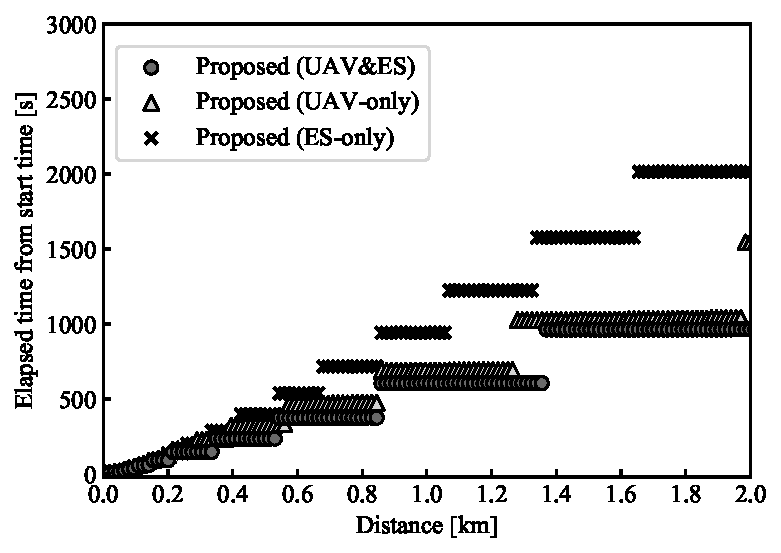
\includegraphics[width=9.0cm]{fig/proposed1.pdf}
\caption{Elapsed time from start time vs. Distance of sensing sections. Proposed (UAV\&ES), Proposed (UAV-only), and Proposed (ES-only) are compared.}
\label{1}
\end{center}
\end{figure}

\begin{figure}[t]
\begin{center}
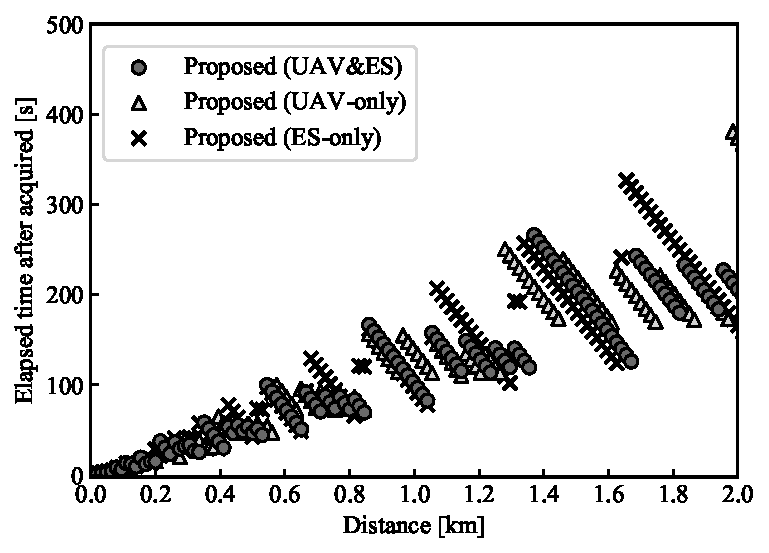
\includegraphics[width=9.0cm]{fig/proposed2.pdf}
\caption{Elapsed time after acquired vs. Distance of sensing sections. Proposed (UAV\&ES), Proposed (UAV-only), and Proposed (ES-only) are compared.}
\label{2}
\end{center}
\end{figure}

Figure \ref{1} plots the elapsed time from the start time about each image versus the distance of the sensing section at which the image is acquired from the initial position.
%
As we see in the figure, the elapsed times in all the proposed methods keep almost constant and then increase for the longer distance of sensing sections.
%
However, Proposed (ES-only) worked a little worse than Proposed (UAV\&ES) and Proposed (UAV-only) in terms of this metric.

On the other hand, Figure \ref{2} plots the elapsed time after acquired about each image.
%
The horizontal axis of this figure is the same as the one in Figure \ref{1}.
%
In this figure, the elapsed time after acquired decreases with some regular pattern, against the distance of the sensing sections.
%
In a part of the areas:0.25-0.35km, 0.65-0.75km, 0.85-0.90km, 1.2-1.4km, 1.9-2.0km, Proposed (ES-only) and Proposed (UAV-only) worked better than Proposed (UAV\&ES) in terms of this metric.
On the other hand, in all the rest areas (most of the whole areas), Proposed (UAV\&ES) worked better than Proposed (UAV-only) and Proposed (ES-only).

From the above result, the proposed method is adaptable to various situations of given computational performance.
It also suggests that Proposed (UAV\&ES) worked best among the three types of computing using the proposed scheduling methods thanks to its integrated computational power of UAVs and the ES. 
%
There, in the next section, we only focus on Proposed (UAV\&ES) without considering Proposed (UAV-only) and Proposed (ES-only).

\subsubsection{Comparison with fixed method}

\begin{figure}[t]
\begin{center}
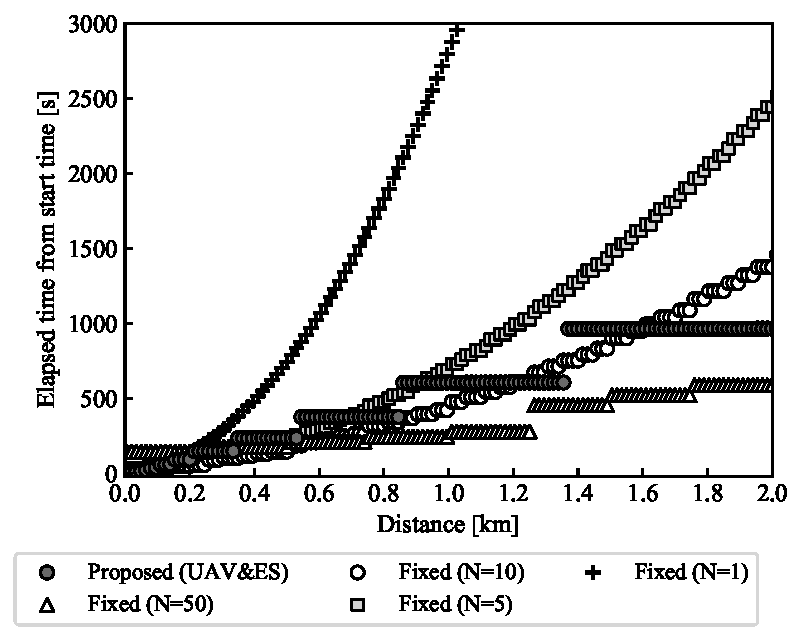
\includegraphics[width=9.0cm]{fig/compared1.pdf}
\caption{Elapsed time from start time vs. Distance of sensing sections. Proposed and Fixed are compared.}
\label{3}
\end{center}
\end{figure}

\begin{figure}[t]
\begin{center}
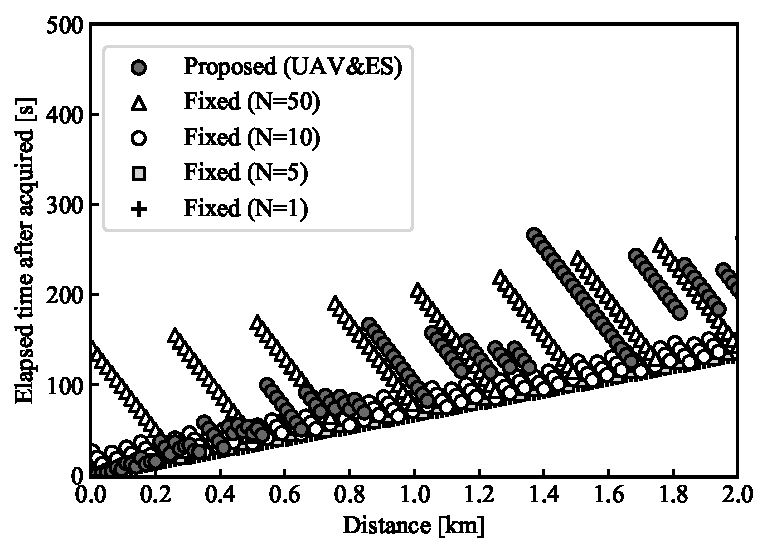
\includegraphics[width=9.0cm]{fig/compared2.pdf}
\caption{Elapsed time after acquired vs. Distance of sensing sections. Proposed and Fixed are compared.}
\label{4}
\end{center}
\end{figure}

In this section, we compare Proposed (UAV\&ES) with Fixed defined in Section \ref{compare}.
%
The vertical and horizontal axes in Figures \ref{3} and \ref{4} are the same as the ones in Figures \ref{1} and \ref{2}, respectively.
%
We examined the Fixed with $N^i$ = 1, 5, 10, and 50.

%
In Figure \ref{3}, for longer distance of sensing sections, the elapsed time from start time monotonically increases in all the methods.
%
However, in the Fixed, as $N^i$ was set larger, the elapsed time increased more gradually.
%
Proposed (UAV\&ES) performed similarly to the Fixed with $N^i=10$.

On the other hand, in Figure \ref{4}, the elapsed time after acquired decreases with some regular pattern in all the methods.
%
However, in the Fixed, as $N^i$ was set smaller, the elapsed time became shorter.
%
Proposed (UAV\&ES) worked between the Fixed with $N^i=10$ and $N^i=50$.

From the overall observation shown above, in the Fixed, $N^i=10$ should be most reasonable in terms of both types of elapsed time.
%
Since Proposed (UAV\&ES) worked similarly to the Fixed with $N^i=10$ without requiring any parameter setting unlike the Fixed, we can conclude that Proposed (UAV\&ES) works best in this evaluation scenario.


\section{Extension to two-dimensional model}\label{twodi}
%Note that the proposed scheduling method described in Section \ref{math} is applicable to the one-dimensional model shown in Figure  \ref{model1.5}.
In this section, we mention that the proposed scheduling method described in Section \ref{math} can be applied not only to the one-dimensional model in Figure \ref{model1.5} but also directly to the two-dimensional model.
There are two assumptions in which the proposed scheduling method can be extended to the two-dimensional model shown in Figure \ref{twodimention} :

\begin{description}
%\item[(1)] 扇型のsensing regionを仮定し、各区画範囲が一定となるように分割
\item[(1)]  Assuming fan-shaped sensing region, split the region so that each sensing section range is constant
%幅$d$のリング上に区切った後、各区画範囲が$\frac{1}{2}d^2\theta$で一定となるように分割
%\item[(2)]文献\cite{Maza2007}と同様に各UAVはジグザク上に中心に近い領域から順にセンシングを実行
\item[(2)] Each UAV executes sensing on the zigzag in order from the area closest to the center like \cite{Maza2007}
\end{description}

%Figure  \ref{twodimention} に示すように,各区画の縦幅を$d$,扇型領域の中心角を$\theta$ [rad]とした時,
As shown in Figure \ref{twodimention}, assuming that the vertical width of each partition is $d$ and the central angle of the sensing region is $\theta$ [rad], the distance between each section when UAV moves in the direction opposite to the center of the region is $d$ and the distance between each section when moving on the circumference is $\frac{1}{2}d\theta$.
%UAVが縦に移動する際の区画間距離は$d$,横に移動する際の区画間距離は$\frac{1}{2}d\theta$となる.
%よって$\theta=2$ [rad]の時,the one-dimensional model shown in Figure  \ref{model1.5}と同様に区画間距離は全て等しくなるので,the proposed scheduling method described in Section \ref{math}をそのまま適用することが可能となる.
Therefore, when $\theta=2$ [rad], all the distance between each section are equal as in Figure \ref{model1.5} and the proposed scheduling method described in Section \ref{math} can be directly applicable to the Figure \ref{twodimention}.
\begin{figure}[t]
\begin{center}
\includegraphics[width=6.0cm]{fig/twodimention.eps}
\caption{Sensing region of two-dimensional model}
\label{twodimention}
\end{center}
\end{figure}

\section{CONCLUSION}
This paper proposed a scheduling method of multi-UAV search system that considers processing time of the acquired image data and data transfer time in areas where humans and ground vehicles cannot easily step into like disaster-damaged areas.
In this paper, we first showed the system model, which consists of a user device, multiple UAVs, and an edge server, and mentioned the sytem flow. 
We then presented the problem formulation of the proposed scheduling method that maximizes the user’s utility, which is calculated from the efficiency of obtaining results from analyzed data and the interval of obtaining the results, by using the one-dimensional model where sensing sections are placed on the one-dimensional line and their sizes are identical.
A simulation was performed to verify that the proposed method works well to ensure the freshness of individual obtained piece of information while delivering as many pieces of information as possible for a certain period.
The results indicated that the proposed method works better than the conventional fixed methods, in terms of two metrics: i) elapsed time from start time and ii) elapsed time after acquired for each image.
For a more practical evaluation, in our future work, we will include prototype implementation and experiment.

%\bibitem{Pitre2012} R. R. Pitre, X. R. Li, R. Delbalzo, “UAV Route Planning for Joint
%Search and Track Missions-An Information-Value Ap-proach”,  \emph{IEEE
%Trans. Aerospace and Electronic Systems}, vol. 48, no.3, pp.2551 -2565, 2012

% if have a single appendix:
%\appendix[Proof of the Zonklar Equations]
% or
%\appendix  % for no appendix heading
% do not use \section anymore after \appendix, only \section*
% is possibly needed

% use appendices with more than one appendix
% then use \section to start each appendix
% you must declare a \section before using any
% \subsection or using \label (\appendices by itself
% starts a section numbered zero.)
%


\appendices
\section{optimal solution}\label{ape}
This section discusses a solution of the problem formulation described in section \ref{math}, which is used in our scheduling method.
%
It takes long time to solve formulas (\ref{eq1}) and (\ref{eq2}) due to their computational complexities, the calculation for scheduling could be non-negligible overhead in the system; UAVs have to wait to start flying until their schedules have been determined.
%
%We need to solve the optimization problem of formula (\ref{eq1}), (\ref{eq2}) for all UAVs in as short a time as possible.
%
%However, if we consider the influence of UAV${i-1}$ or earlier, that is, wait time $T_{u,d}^{i}(N^i,N_u^i)$, $T_{d,e}^{i}(N^i,N_u^i)$, $T_e^{i}(N^i,N_u^i)$ in ${t_{fin}^i}$, $\frac{\eta^i}{{\Delta{t}}^i}$ becomes complicated and we have difficulty solving the optimization problem of formula (\ref{eq1}), (\ref{eq2}) for all UAVs in realistic time.
Therefore, to simplify the calculation of formulas (\ref{eq1}) and (\ref{eq2}), our scheduling method first supposes that all the waiting times for UAV $i$ are equal to zero and obtains an approximated solution, $N_{th}^i$.
Then, by searching locally around $N_{th}^i$, our scheduling method considers all the waiting times in formulas (\ref{eq1}) and (\ref{eq2}) and finds out the local optimal solution, $N_{l}^i$.
The following part explains the way of finding out $N_{th}^i$.
%
First, we set all the waiting times to zero.
%
Then, we replace the second and fourth terms in formula (\ref{eq_fin}) with $2F$ and $M$, respectively.
%
Then, by substituting ${t_{fin}^i}$ in (\ref{eq_fin}) to formula (\ref{ut}), we obtain $\frac{\eta^i}{{\Delta{t}}^i}$ as below:
%
\begin{align}
\frac{\eta^{i}}{{\Delta{t}}^i}
=&\frac{N^i}{N^i({T_g}+T_{ng})+2F+M}\times\nonumber\\
&\frac{1}{N^i({T_g}+T_{ng})+2F+M+t_{start}^i-t_{fin}^{i-1}}\label{eq4}
\end{align}
%
where, by regarding $N^i$ as a constant, only $M$ is a variable and the value of $\frac{\eta^{i}}{{\Delta{t}}^i}$ varies dependently on the values of $N_u^i$ and $N_e^i$.
%
Since $\frac{\eta^{i}}{{\Delta{t}}^i}$ is always positive,  $M$ takes the minimum when $\frac{\eta^{i}}{{\Delta{t}}^i}$ takes the maximum. 
%
Although $N^i$, $N_u^i$, and $N_e^i$ are integers, here we deal with them as real numbers.
%
Considering $N^i=N_u^i + N_e^i$, on the assumption that $\frac{N_u^i}{P_u^i}$ equals to $\frac{N_e^i}{\mu_{u,d}}+\frac{N_e^i}{\mu_{d,e}}+\frac{N_e^i}{P_e}$, we can obtain the value of $N_u^i$ and $N_e^i$ that satisfy $0\leq{N_u^i}$ and ${N_e^i}\leq{N^i}$ as follows:
%
\begin{align}
N_u^i=\frac{P_u^i(\mu_{d,e}P_e+\mu_{u,d}P_e+\mu_{u,d}\mu_{d,e})}{\mu_{u,d}\mu_{d,e}P_e+P_u^i(\mu_{d,e}P_e+\mu_{u,d}P_e+\mu_{u,d}\mu_{d,e})}N^i\label{eq5}\\
N_e^i=\frac{\mu_{u,d}\mu_{d,e}P_e}{\mu_{u,d}\mu_{d,e}P_e+P_u^i(\mu_{d,e}P_e+\mu_{u,d}P_e+\mu_{u,d}\mu_{d,e})}N^i\label{eq6}
\end{align}
%
When $M$ takes the minimum value, $\frac{N_u^i}{P_u^i}$ is theoretically equal to $\frac{N_e^i}{\mu_{u,d}}+\frac{N_e^i}{\mu_{d,e}}+\frac{N_e^i}{P_e}$, while $N_u^i$ and $N_e^i$ become formula (\ref{eq5}) and (\ref{eq6}), respectively.
%
As $N^i$ becomes larger, $\frac{N_u^i}{P_u^i}$ is closer to $\frac{N_e^i}{\mu_{u,d}}+\frac{N_e^i}{\mu_{d,e}}+\frac{N_e^i}{P_e}$.
%
Thus, $\frac{N_u^i}{P_u^i}=\frac{N_e^i}{\mu_{u,d}}+\frac{N_e^i}{\mu_{d,e}}+\frac{N_e^i}{P_e}$ is established.\\
%
As a result, $\frac{\eta^{i}}{{\Delta{t}}^i}$ in formula (\ref{eq4}) is given as:
%
\begin{align}
&\hspace{-0.2cm}\frac{N^i}{R^2{(N^i)}^2+(4F+t_{start}^i-t_{fin}^{i-1})R{N^i}+2F(2F+t_{start}^i\hspace{-1mm}-t_{fin}^{i-1})}\hspace{1cm}\label{eq_ec}\\
&\hspace{-0.6cm}\biggl(R=T_g+T_{ng}+\frac{\mu_{d,e}P_e+\mu_{u,d}P_e+\mu_{u,d}\mu_{d,e}}{\mu_{u,d}\mu_{d,e}P_e+P_u^i(\mu_{d,e}P_e+\mu_{u,d}P_e+\mu_{u,d}\mu_{d,e})}\biggr)\nonumber
\end{align}
%
To sketch formula (\ref{eq_ec}), by differentiating it by $N^i$, we obtain:
%
\begin{align}
\hspace{-4mm} \frac{-{R^2{(N^i)}^2}+2F(2F+t_{start}^i\hspace{-1mm}-t_{fin}^{i-1})}{\{R^2{(N^i)}^2+(4F+t_{start}^i\hspace{-1mm}-t_{fin}^{i-1})R{N^i}+2F(2F+t_{start}^i\hspace{-1mm}-t_{fin}^{i-1})\}^2}
\end{align}
%
When $t_{start}^i \leq{t_{fin}^{i-1}-2F}$, formula (\ref{eq_ec}) decreases monotonically as the value of $N^i$ increases and takes the maximum when $N_{th}^i$ is $N_{MIN}^i$.
%
When $t_{start}^i >{t_{fin}^{i-1}-2F}$, $\frac{\eta^{i}}{{\Delta{t}}^i}$ is a convex function taking the maximum when $N^i$ is $\frac{\sqrt{2F(2F+t_{start}^i-t_{fin}^{i-1})}}{R}$.
%
Note that $N^i$ is chosen so that the denominator of formula (\ref{eq_ec}) does not become zero.
%
Through the above procedures, we can obtain $N_{th}^i$ as follows:
%
\begin{align}
 \hspace{-1.5mm} N_{th}^i= \begin{cases}
    \frac{\sqrt{2F(2F+t_{start}^i-t_{fin}^{i-1})}}{R} & ({N_{MIN}^i}\leq{\frac{\sqrt{2F(2F+t_{start}^i-t_{fin}^{i-1})}}{R}}) \\
    N_{MIN}^i& (\frac{\sqrt{2F(2F+t_{start}^i-t_{fin}^{i-1})}}{R}<{N_{MIN}^i})
  \end{cases}
\end{align}

% you can choose not to have a title for an appendix
% if you want by leaving the argument blank
%\section{}
%Appendix two text goes here.


% use section* for acknowledgment
\section*{Acknowledgment}
This work was partly supported by JSPS KAKENHI Grant Number JP17H01732.

% Can use something like this to put references on a page
% by themselves when using endfloat and the captionsoff option.
\ifCLASSOPTIONcaptionsoff
  \newpage
\fi

% trigger a \newpage just before the given reference
% number - used to balance the columns on the last page
% adjust value as needed - may need to be readjusted if
% the document is modified later
%\IEEEtriggeratref{8}
% The "triggered" command can be changed if desired:
%\IEEEtriggercmd{\enlargethispage{-5in}}

% references section

% can use a bibliography generated by BibTeX as a .bbl file
% BibTeX documentation can be easily obtained at:
% http://mirror.ctan.org/biblio/bibtex/contrib/doc/
% The IEEEtran BibTeX style support page is at:
% http://www.michaelshell.org/tex/ieeetran/bibtex/
%\bibliographystyle{IEEEtran}
% argument is your BibTeX string definitions and bibliography database(s)
%\bibliography{IEEEabrv,../bib/paper}
%
% <OR> manually copy in the resultant .bbl file
% set second argument of \begin to the number of references
% (used to reserve space for the reference number labels box)
\begin{thebibliography}{1}
\bibitem{CRED2016}Debarati Guha-Sapir, Philippe Hoyois, Pasacline Wallemacq and Regina Below,``Annual Disaster Statistical Review 2016,"\emph{Centre for Research on
the Epidemiology of Disasters},2016 
\bibitem{disaster2011} Japan Ministry of Defense, ``Lessons from the Great East Japan Earthquake," \url{http://www.mod.go.jp/e/publ/w_paper/pdf/2012/30_Part3_Chapter1_Sec3.pdf}, 2012
\bibitem{Andre2014} T. Andre, K. Hummel, A. Schoellig, E. Yanmaz, M. Asadpour, C. Bettstetter, P. Grippa, H. Hellwagner, S. Sand and S. Zhang, ``User devicelication-driven design of aerial communication networks, " \emph{IEEE Commun. Mag.}, vol. 52, no. 5, pp. 129-137, 2014
\bibitem{Erdelj2016} M. Erdelj, and N. Enrico, ``UAV-assisted disaster management: User devicelications and open issues, " \emph{2016 International Conference on Computing, Networking and Communications (ICNC)},pp1-5, 2016
\bibitem{Felice2014} M. Di Felice, A. Trotta, L. Bedogni, K. R. Chowdhury and L. Bononi, ``Self-organizing aerial mesh networks for emergency communication, " \emph{Personal, Indoor, and Mobile Radio Communication (PIMRC), IEEE 25th Annual International Symposium on}, pp. 1631-1636, 2014
\bibitem{japan2011}Armand Vervaeck and James Daniell,``Japan Tohoku tsunami and earthquake : The death toll is climbing again!, " \url{https://earthquake-report.com/2011/08/04/japan-tsunami-following-up-the-aftermath-part-16-june/}, 2011
\bibitem{Lanillos2014} P. Lanillos, S. K. Gan, E. Besada-Portas, G. Pajares and S. Sukkarieh, ``Multi-UAV target search using decentralized gradient-based negotiation with expected observation,"\emph{Information Sciences}, vol. 282, pp. 92-110, 2014.
\bibitem{Maza2007} I. Maza, A. Ollero, ``Multiple UAV cooperative searching operation
using polygon area decomposition and efficient coverage algorithms, "\emph{Distributed Autonomous Robotic Sys-tems}, pp. 221-230, 2007.
\bibitem{Meng2014} W. Meng, Z. R. He, R. Teo, L. xie, ``Decentralized Search, Tasking and Tracking Using Multiple Fixed-Wing Miniature UAVs," \emph{11th IEEE
International Conference on Control \& Automation (ICCA)}, pp. 1345-1350, 2014 
\bibitem{chang2016} C. Zhao, M. Zhu and H. Liang, ``The Sustainable Tracking Strategy of Moving Target by Multi-UAVs in an Uncertain Environment, " \emph{2016 IEEE/CSAA International Conference on Aircraft Utility Systems (AUS)}, pp. 20-25, 2016
\bibitem{Mirzaei2011} M. Mirzaei, F. Sharifi, B. W. Gordon, C. A. Rabbath and  Y. M.Zhang, ``Cooperative multi-vehicle search and coverage problem in uncertain environments, "\emph{in Proceedings of the 50th IEEE Conference on Decision and Control and European Control Conference (CDCECC)}, pp. 4140-4145, 2011
%
\bibitem{Bamburry2015} D. Bamburry, ``Drones: Designed for product delivery," \emph{Design Management Review}, vol. 26, no. 1, pp. 40-48, 2015
\bibitem{May2015}K. May,``Drones to deliver medicine and food? Drones for disaster relief? Why not?,"\url{https://ideas.ted.com/6-ways-drones-can-be-used-for-good/}, 2013
\bibitem{Wada2015}A. Wada, T. Yamashita, M. Maruyama, T. Arai, H. Adachi and H. Tsuji, ``A surveillance system using small unmanned aerial vehicle (UAV) related technologies,’’\emph{NEC Technical Journal},vol.8, no. 1, p68-72, 2015
\bibitem{Bekmezci2013} I. Bekmezci, O. K. Sahingoz, and S. Temel, “Flying Ad-Hoc Networks (FANETs): a survey,” \emph{Ad Hoc Networks}, vol. 11, no. 3, pp. 1254-1270, 2013
\bibitem{Garcia2016} J S\'anchez-Garc\'ia, JM Garc\'ia-Campos, SL Toral, DG Reina and F Barrero, ``An intelligent strategy for tactical movements of UAVs in disaster scenarios,’’\emph{
International Journal of Distributed Sensor Networks}, vol.12, no. 3, 2016
\bibitem{Hayat 2017}S. Hayat, E. Yanmaz, T. X. Brown, and C. Bettstetter,``Multi-Objective UAV Path Planning for Search and Rescue,” \emph{ICRA Singapore}, 2017 
%
%
\bibitem{Ouahouah2017}S. Ouahouah , T. Taleb, J. Song and C. Benzaid, ``Efficient offloading mechanism for UAVs-based value added services," \emph{IEEE International Conference on Communications (ICC)}, 2017
\bibitem{Valentino2018} R. Valentino, W.-S. Jung and Y.-B. Ko,``Opportunistic Computational Offloading System for Clusters of Drones,” \emph{International Conference on Advanced Communications Technology(ICACT)}, 2018 
%\bibitem{Nigam2014} N. Nigam, ``The Multiple Unmanned Air Vehicle Persistent Surveillance Problem: A Review, \emph{Machines}, Vol.2, Issue 1, pp. 13-72, 2014
%\bibitem{Loke2015} S. W. Loke, "The internet of flying-things: Opportunities and challenges with airborne fog computing and mobile cloud in the clouds, " \emph{arXiv preprint arXiv:1507.04492}, 2015
%\bibitem{Jeong2016} S. Jeong, O. Simeone, and J. Kang, "Mobile edge computing via a UAVmounted cloudlet: Optimal bit allocation and path planning, "\emph{IEEE Transactions on Vehicular Technology,to appear}, 2017
\bibitem{Motlagh2017}N. H. Motlagh, M. Bagaa, and T. Taleb, ``Uav-based iot platform: A crowd surveillance use case,\emph{IEEE Communications Magazine}, vol.55, no.2, pp. 128-134, 2017
%\bibitem{Mohamed2017}M.-A. Messous, H. Sedjelmaci, N. Houari, S.-M. Senouci, ``Computation offloading game for an uav network in mobile edge computing,\emph{IEEE International Conference on Communications (ICC)}, pp. 1-6, 2017
\bibitem{Messous2017} M.-A. Messous1, A. Arfaoui, A. Alioua, S. -M. Senouci,``A Sequential Game Approach for Computation-Offloading in an UAV Network,’’\emph{IEEE Global Communications Conference}, 2017 
\bibitem{bebop2} Parrot SA, ``PARROT BEBOP2 SO LIGHT YOU CAN TAKE IT
ANYWHERE TO FILM IN FULL HD, "
\url{http://www.parrot.com/usa/products/bebop2/}, 2016
%\bibitem{UPF614496} ``Lithium Ion UPF614496,'' Panasonic, \url{http://www.panamar.it/images/date_sheets_UPF-614496.pdf}, Jan.20, 2016

%\bibitem{Traub2016} L.W. Traub,  ``Calculation of Constant Power Lithium Battery Discharge Curves,'' \emph{Batteries}, vol2, no2, 2016
\bibitem{Ren2015} S. Ren, K. He, R. Girshick, J. Sun, ``Faster R-CNN: Towards
real-time object detection with region proposal networks,'' \emph{In Advances in neural information processing systems}, pp. 91-99, 2015
\bibitem{Li2013} J. Li, Y. Fan, H. Chen, K. Xu, Y. Dai, F. Yin, Y. Ji,  ``Radio-over-fiber-based distributed antenna systems supporting IEEE 802.11 N/AC standards,'' \emph{Optical Communications and Networks (ICOCN), 2013 12th International Conference on. IEEE}, pp. 1-4, 2013

\end{thebibliography}

% biography section
% 
% If you have an EPS/PDF photo (graphicx package needed) extra braces are
% needed around the contents of the optional argument to biography to prevent
% the LaTeX parser from getting confused when it sees the complicated
% \includegraphics command within an optional argument. (You could create
% your own custom macro containing the \includegraphics command to make things
% simpler here.)
%\begin{IEEEbiography}[{\includegraphics[width=1in,height=1.25in,clip,keepaspectratio]{mshell}}]{Michael Shell}
% or if you just want to reserve a space for a photo:

%\begin{IEEEbiography}{Michael Shell}
%Biography text here.
%\end{IEEEbiography}

% if you will not have a photo at all:
%\begin{IEEEbiographynophoto}{John Doe}
%Biography text here.
%\end{IEEEbiographynophoto}

% insert where needed to balance the two columns on the last page with
% biographies
%\newpage

%\begin{IEEEbiographynophoto}{Jane Doe}
%Biography text here.
%\end{IEEEbiographynophoto}

% You can push biographies down or up by placing
% a \vfill before or after them. The appropriate
% use of \vfill depends on what kind of text is
% on the last page and whether or not the columns
% are being equalized.

%\vfill

% Can be used to pull up biographies so that the bottom of the last one
% is flush with the other column.
%\enlargethispage{-5in}



% that's all folks
\end{document}


